\section{Images}
\label{sec:images}

\subsection{Text wrapping}
\label{sec:images:text_wrapping}

\begin{wrapfigure}{r}{0.5\textwidth}
  \begin{center}
    \vspace{-1\intextsep}
    \hspace*{-.5\columnsep}
    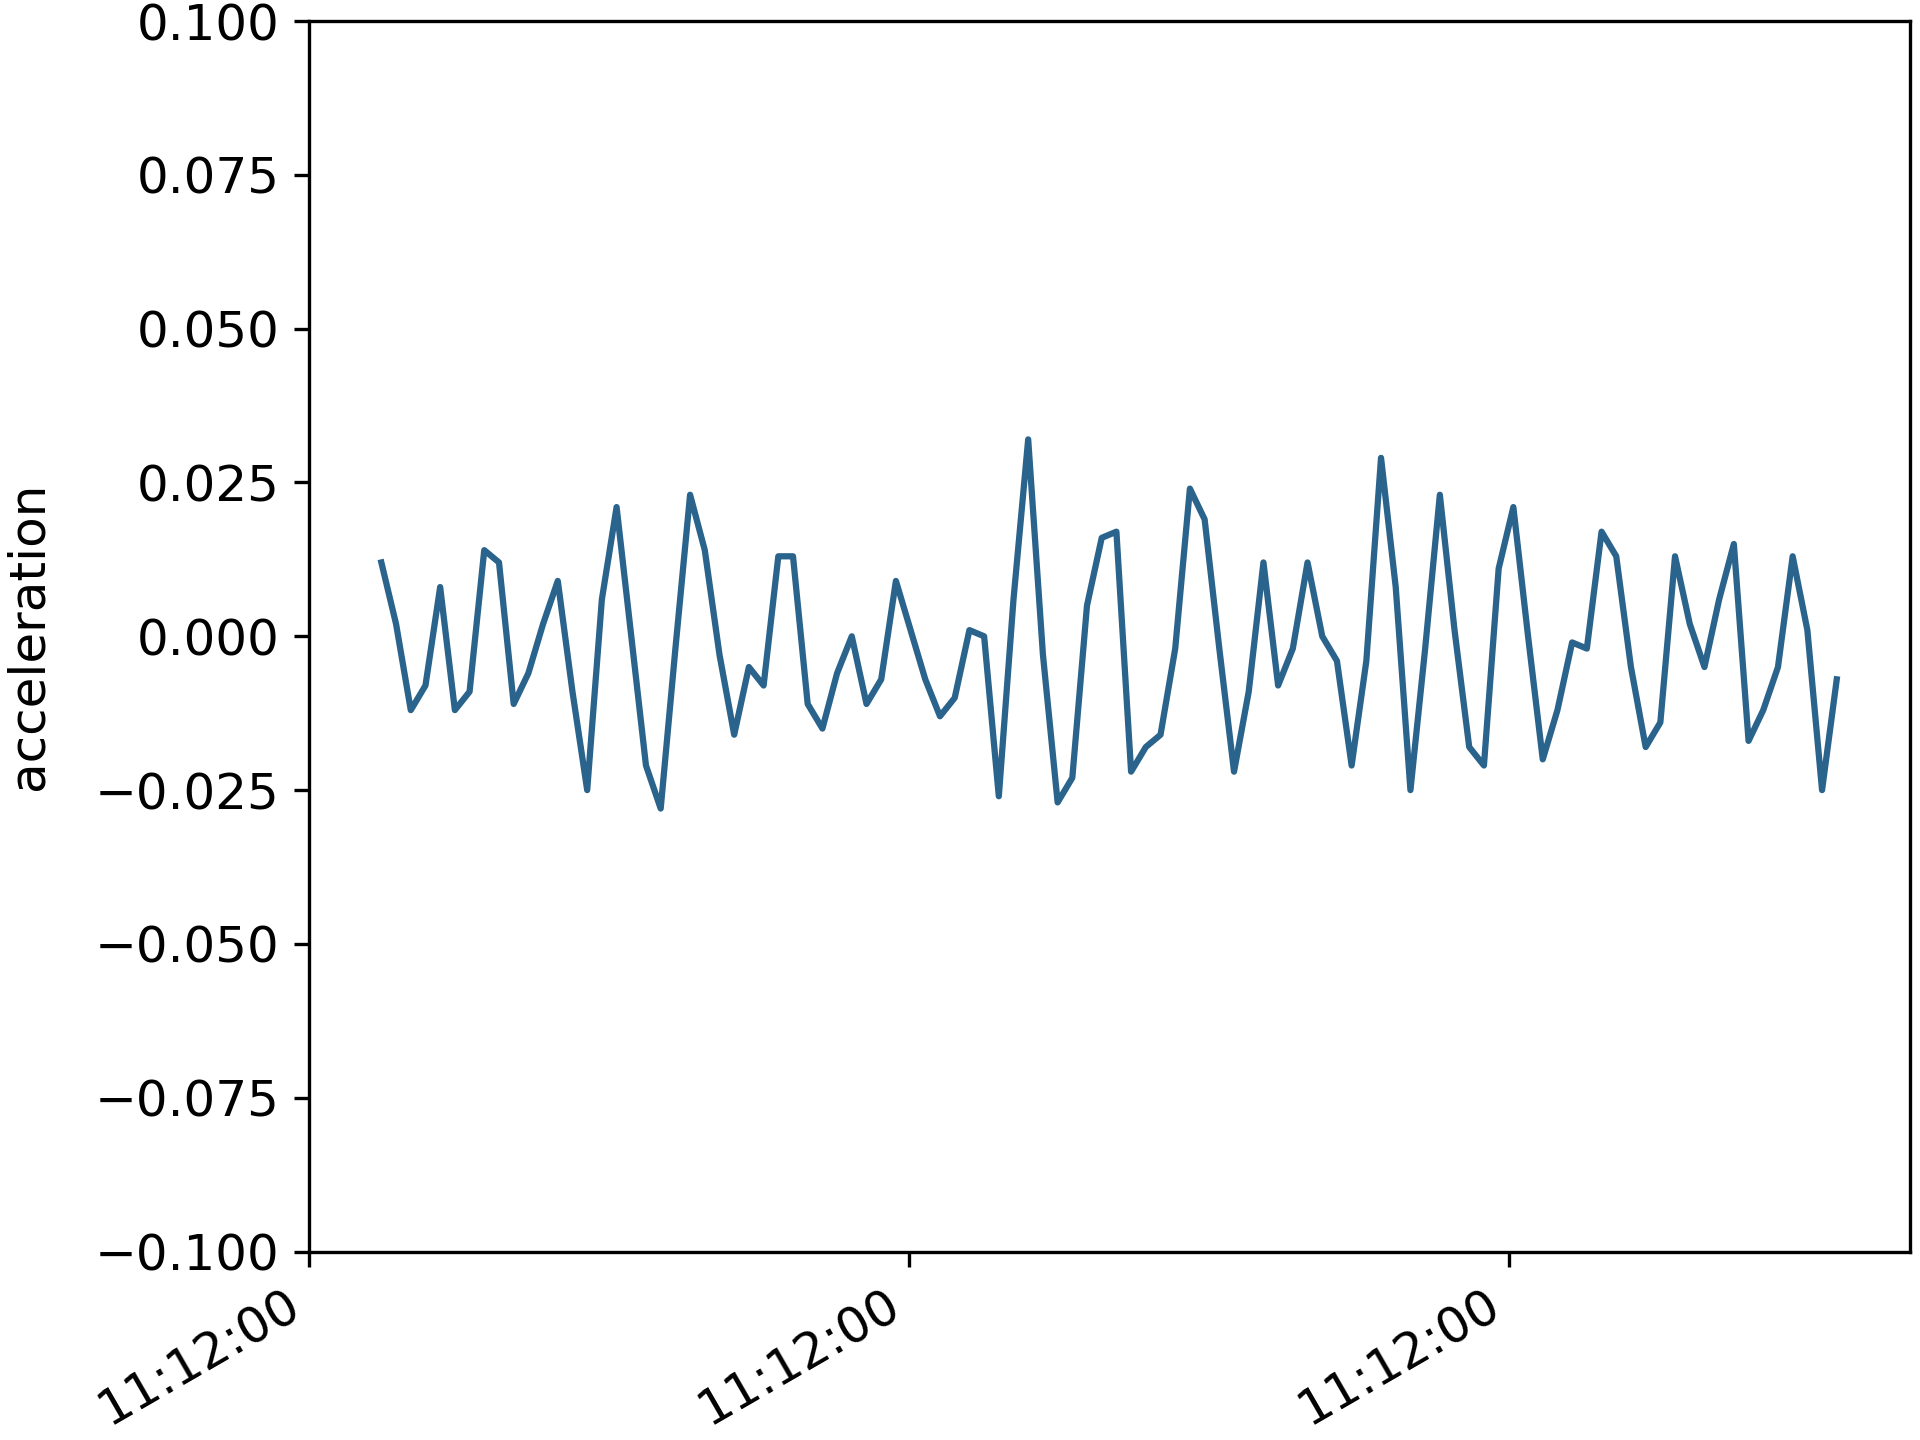
\includegraphics[width=0.5\textwidth]{Resources/Images/Bearing/bearing_acceleration.png}
  \end{center}
  \caption{Bearing acceleration of something}
  \label{fig:images:acceleration}
\end{wrapfigure}

As shown in figure \ref{fig:images:acceleration} lorem ipsum dolor sit amet, consetetur sadipscing elitr, sed diam nonumy eirmod tempor invidunt ut labore et dolore magna aliquyam erat, sed diam voluptua.
At vero eos et accusam et justo duo dolores et ea rebum. Stet clita kasd gubergren, no sea takimata sanctus est Lorem ipsum dolor sit amet.
Lorem ipsum dolor sit amet, consetetur sadipscing elitr, sed diam nonumy eirmod tempor invidunt ut labore et dolore magna aliquyam erat, sed diam voluptua. At vero eos et accusam et justo duo dolores et ea rebum.
Stet clita kasd gubergren, no sea takimata sanctus est Lorem ipsum dolor sit amet. Lorem ipsum dolor sit amet, consetetur sadipscing elitr, sed diam nonumy eirmod tempor invidunt ut labore et dolore magna aliquyam erat, sed diam voluptua.
At vero eos et accusam et justo duo dolores et ea rebum. \cite{example_xy}

\subsection{Centred image}
\label{sec:images:centred_image}

\begin{figure}[H]
	\begin{center}
		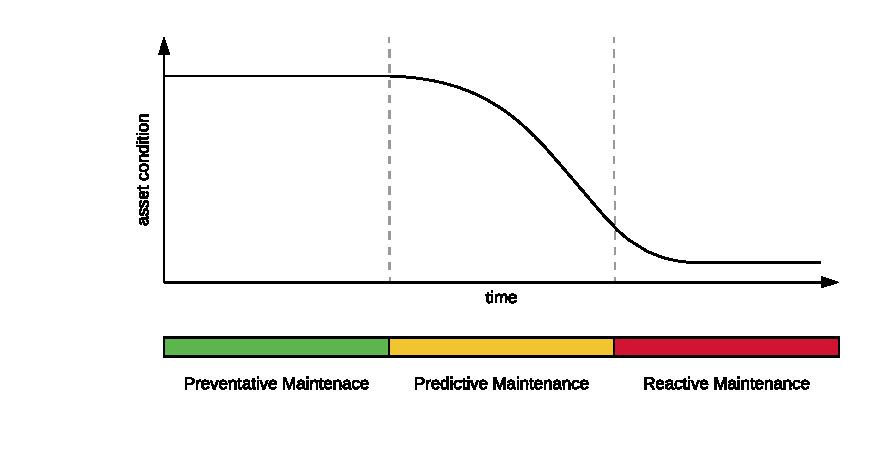
\includegraphics[width=.9\textwidth, clip, trim=1cm 1cm 0.5cm 0.5cm]{Resources/Images/Maintenance/maintenance_types.pdf}
	\end{center}
	\caption{Different types of maintenance}
	\label{fig:images:maintenance_types}
\end{figure}

\subsection{Two images side by side}
\label{sec:images:two_images}

\begin{figure}[H]
	\begin{minipage}{.475\textwidth}
		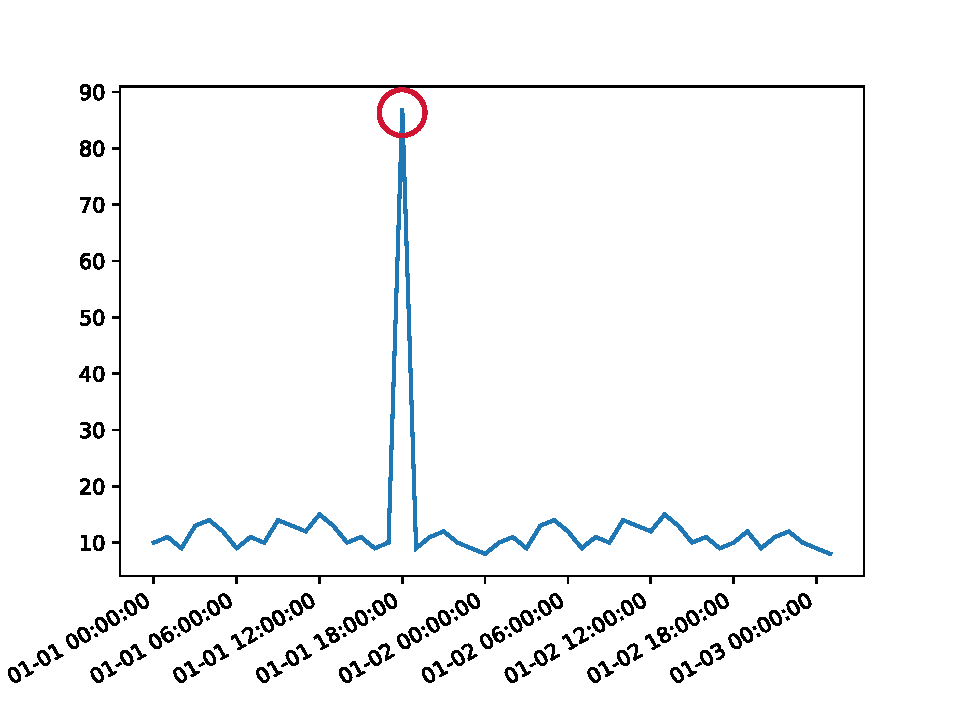
\includegraphics[width=\textwidth, clip, trim=0cm 0.5cm 1cm 1cm]{Resources/Images/Anomalies/point_anomaly.pdf}
		\caption{Point anomaly}
		\label{fig:images:point_anomaly}
	\end{minipage}
	\hspace{0.05\textwidth}
	\begin{minipage}{.475\textwidth}
		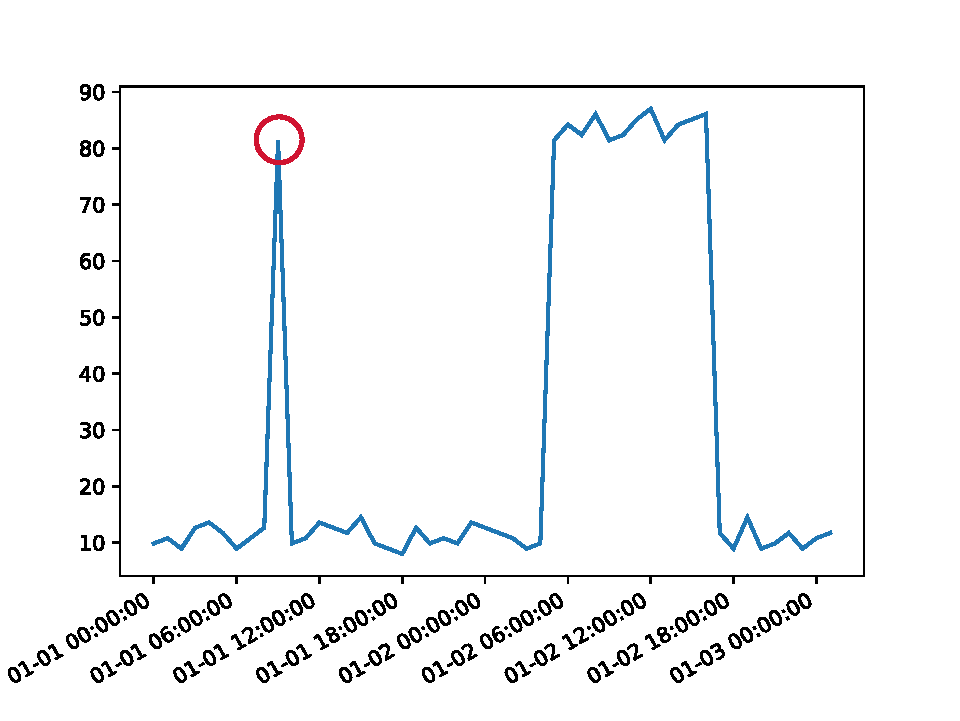
\includegraphics[width=\textwidth, clip, trim=0cm 0.5cm 1cm 1cm]{Resources/Images/Anomalies/contextual_anomaly.pdf}
		\caption{Contextual anomaly}
		\label{fig:images:contextual_anomaly}
	\end{minipage}
\end{figure}


\subsection{Three images side by side (one caption)}
\label{sec:images:three_images}

\begin{figure}[H]
	\begin{tabu} to \textwidth {XXX}
   	\centering\textbf{\footnotesize{Lorem ipsum}} & \centering\textbf{\footnotesize{Dolor sit}} & \centering\textbf{\footnotesize{Amet}} \\
	\end{tabu}
	\begin{minipage}{.325\textwidth}
		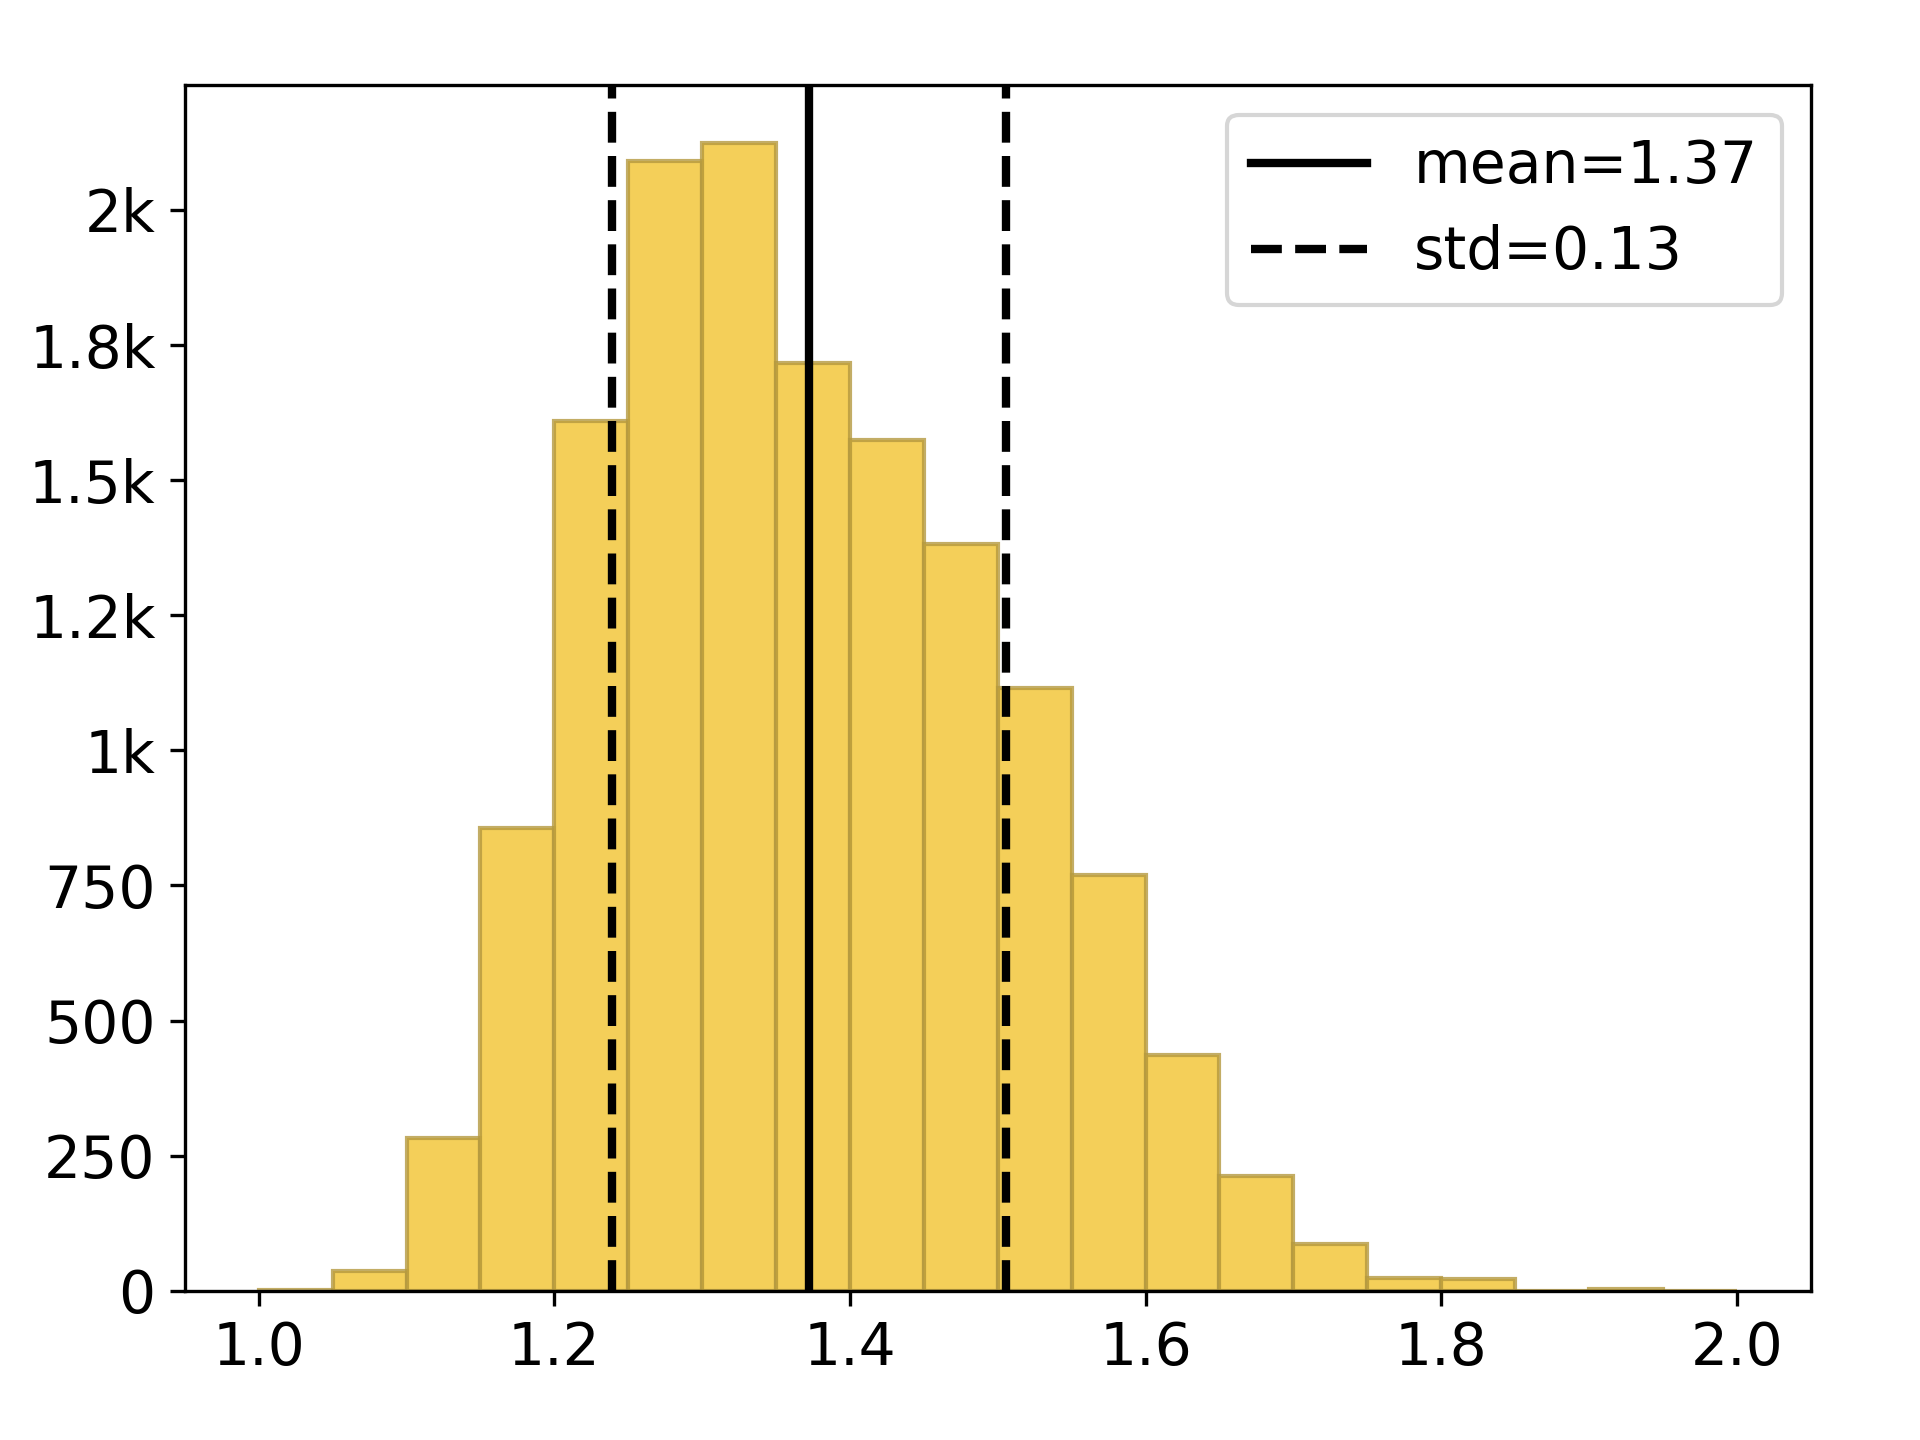
\includegraphics[width=\textwidth, clip,, trim=.25cm 0.25cm .25cm 0.25cm]{Resources/Images/Histogram/hist_1_a.png}
	\end{minipage}
	\begin{minipage}{.325\textwidth}
		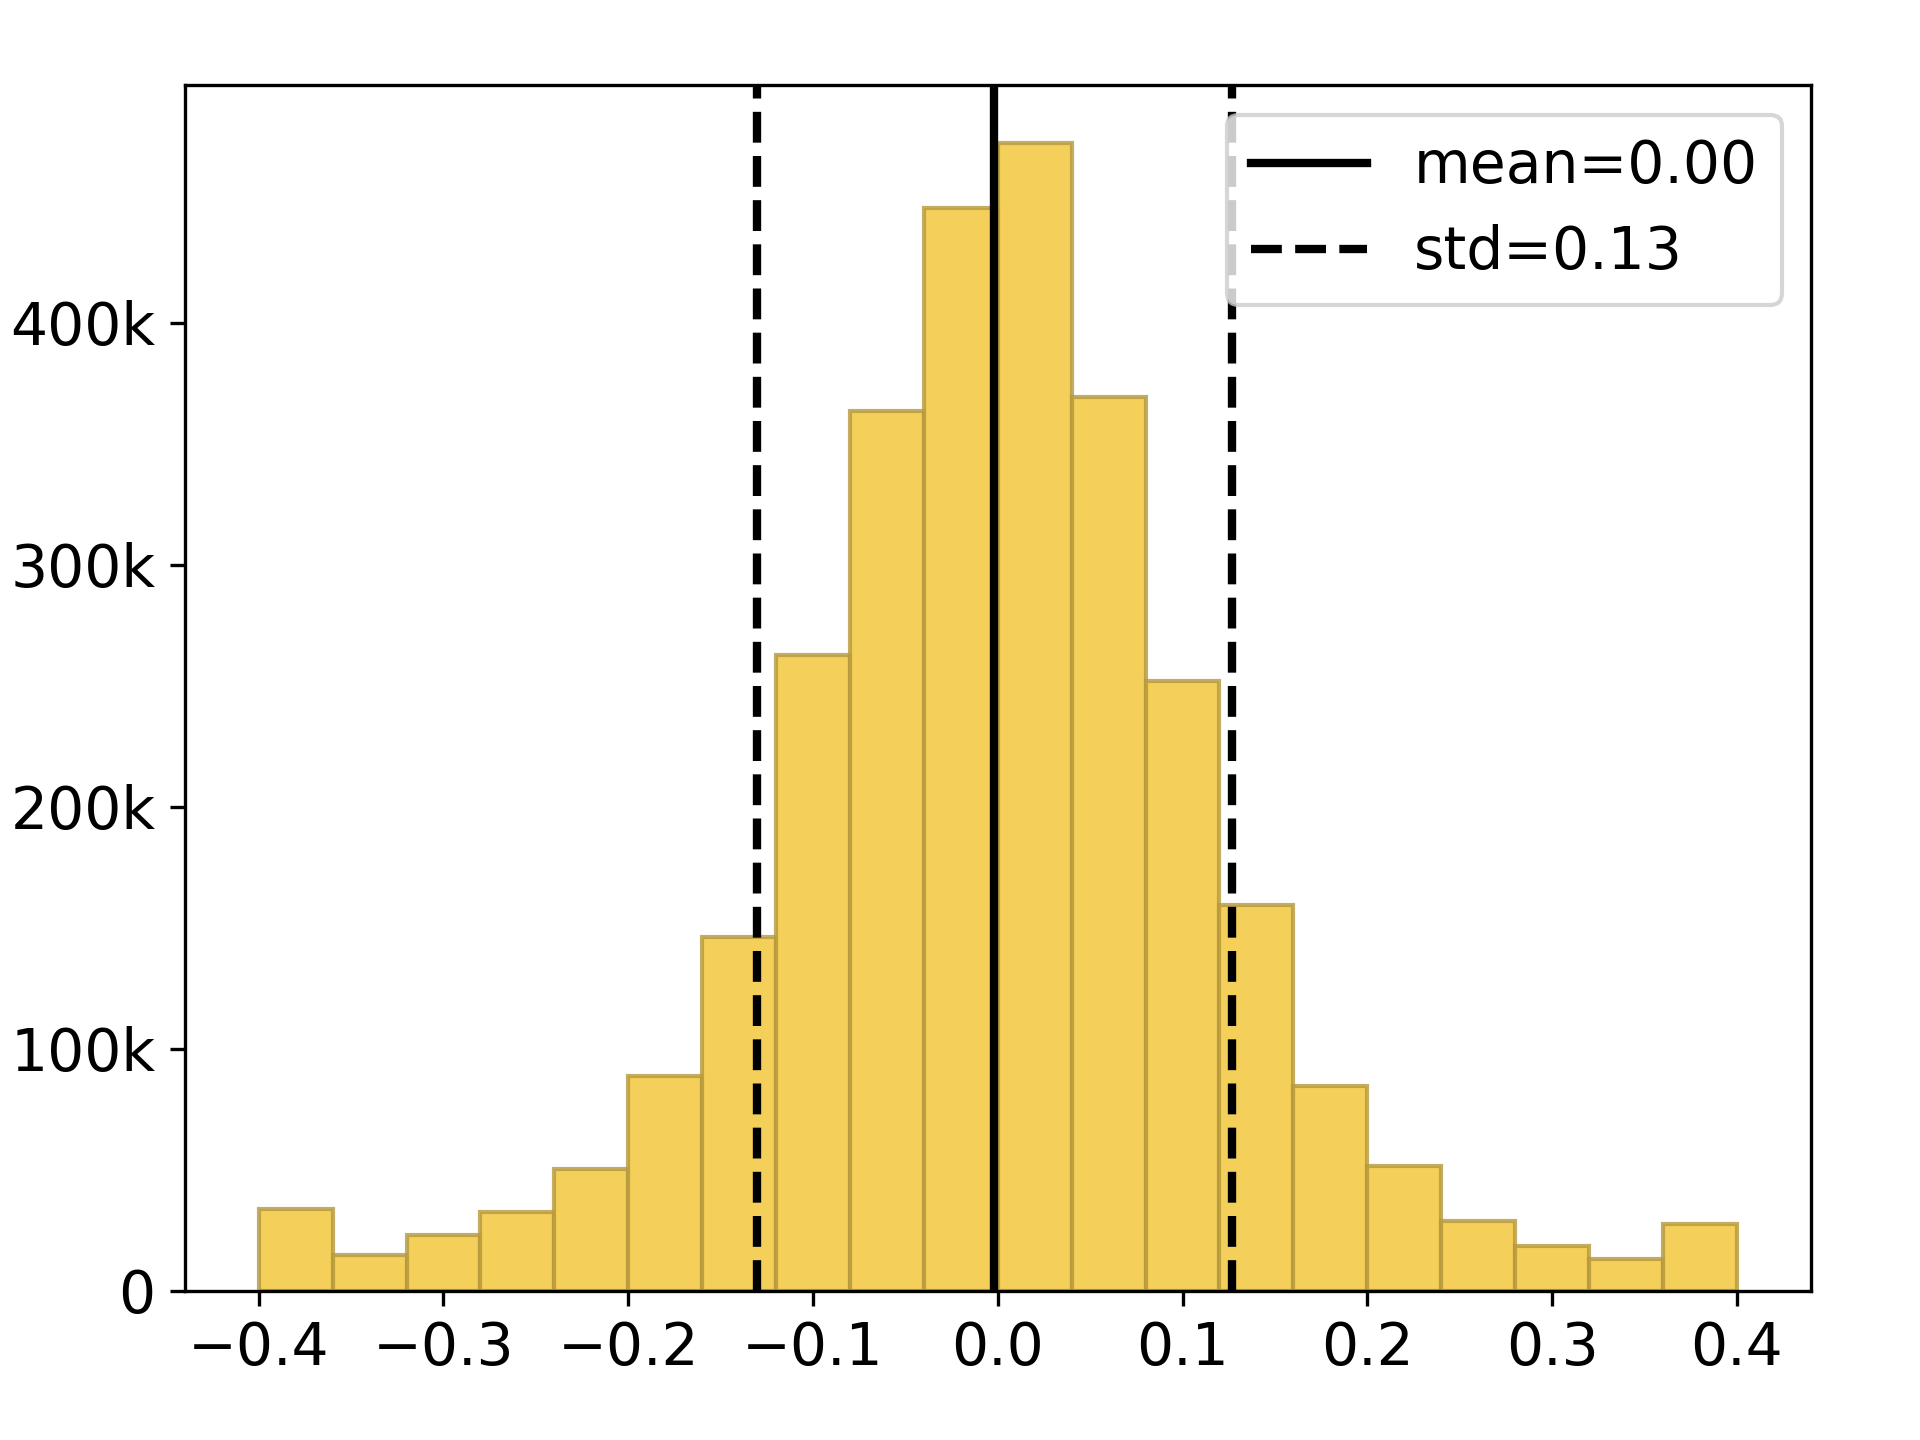
\includegraphics[width=\textwidth, clip, trim=.25cm 0.25cm .25cm 0.25cm]{Resources/Images/Histogram/hist_2_a.png}
	\end{minipage}
	\begin{minipage}{.325\textwidth}
		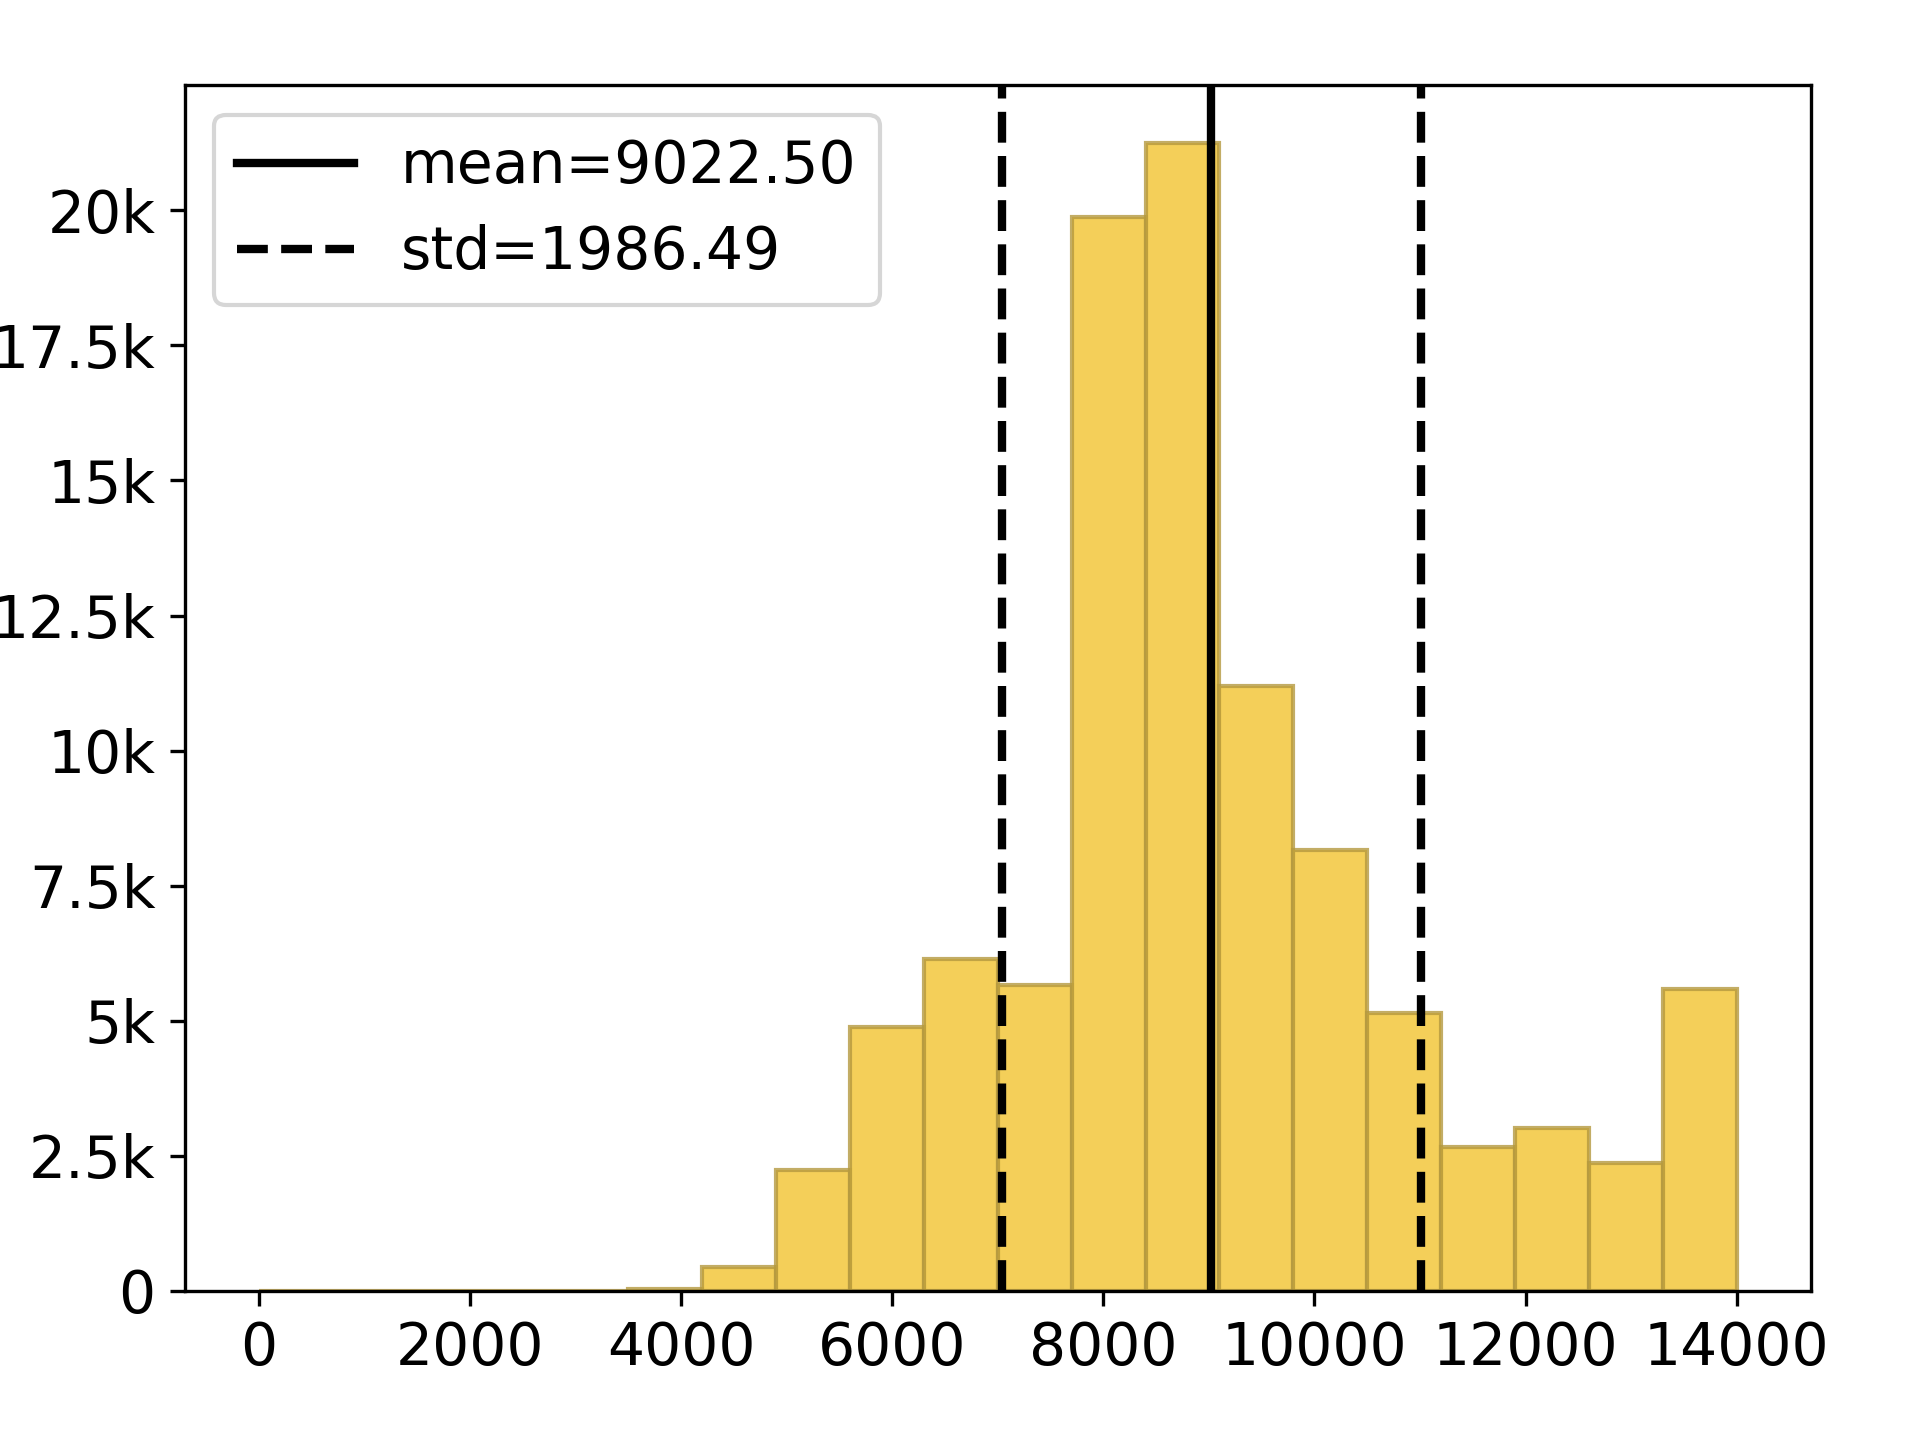
\includegraphics[width=\textwidth, clip, trim=.25cm 0.25cm .25cm 0.25cm]{Resources/Images/Histogram/hist_3_a.png}
	\end{minipage}
	
	\begin{minipage}{.325\textwidth}
		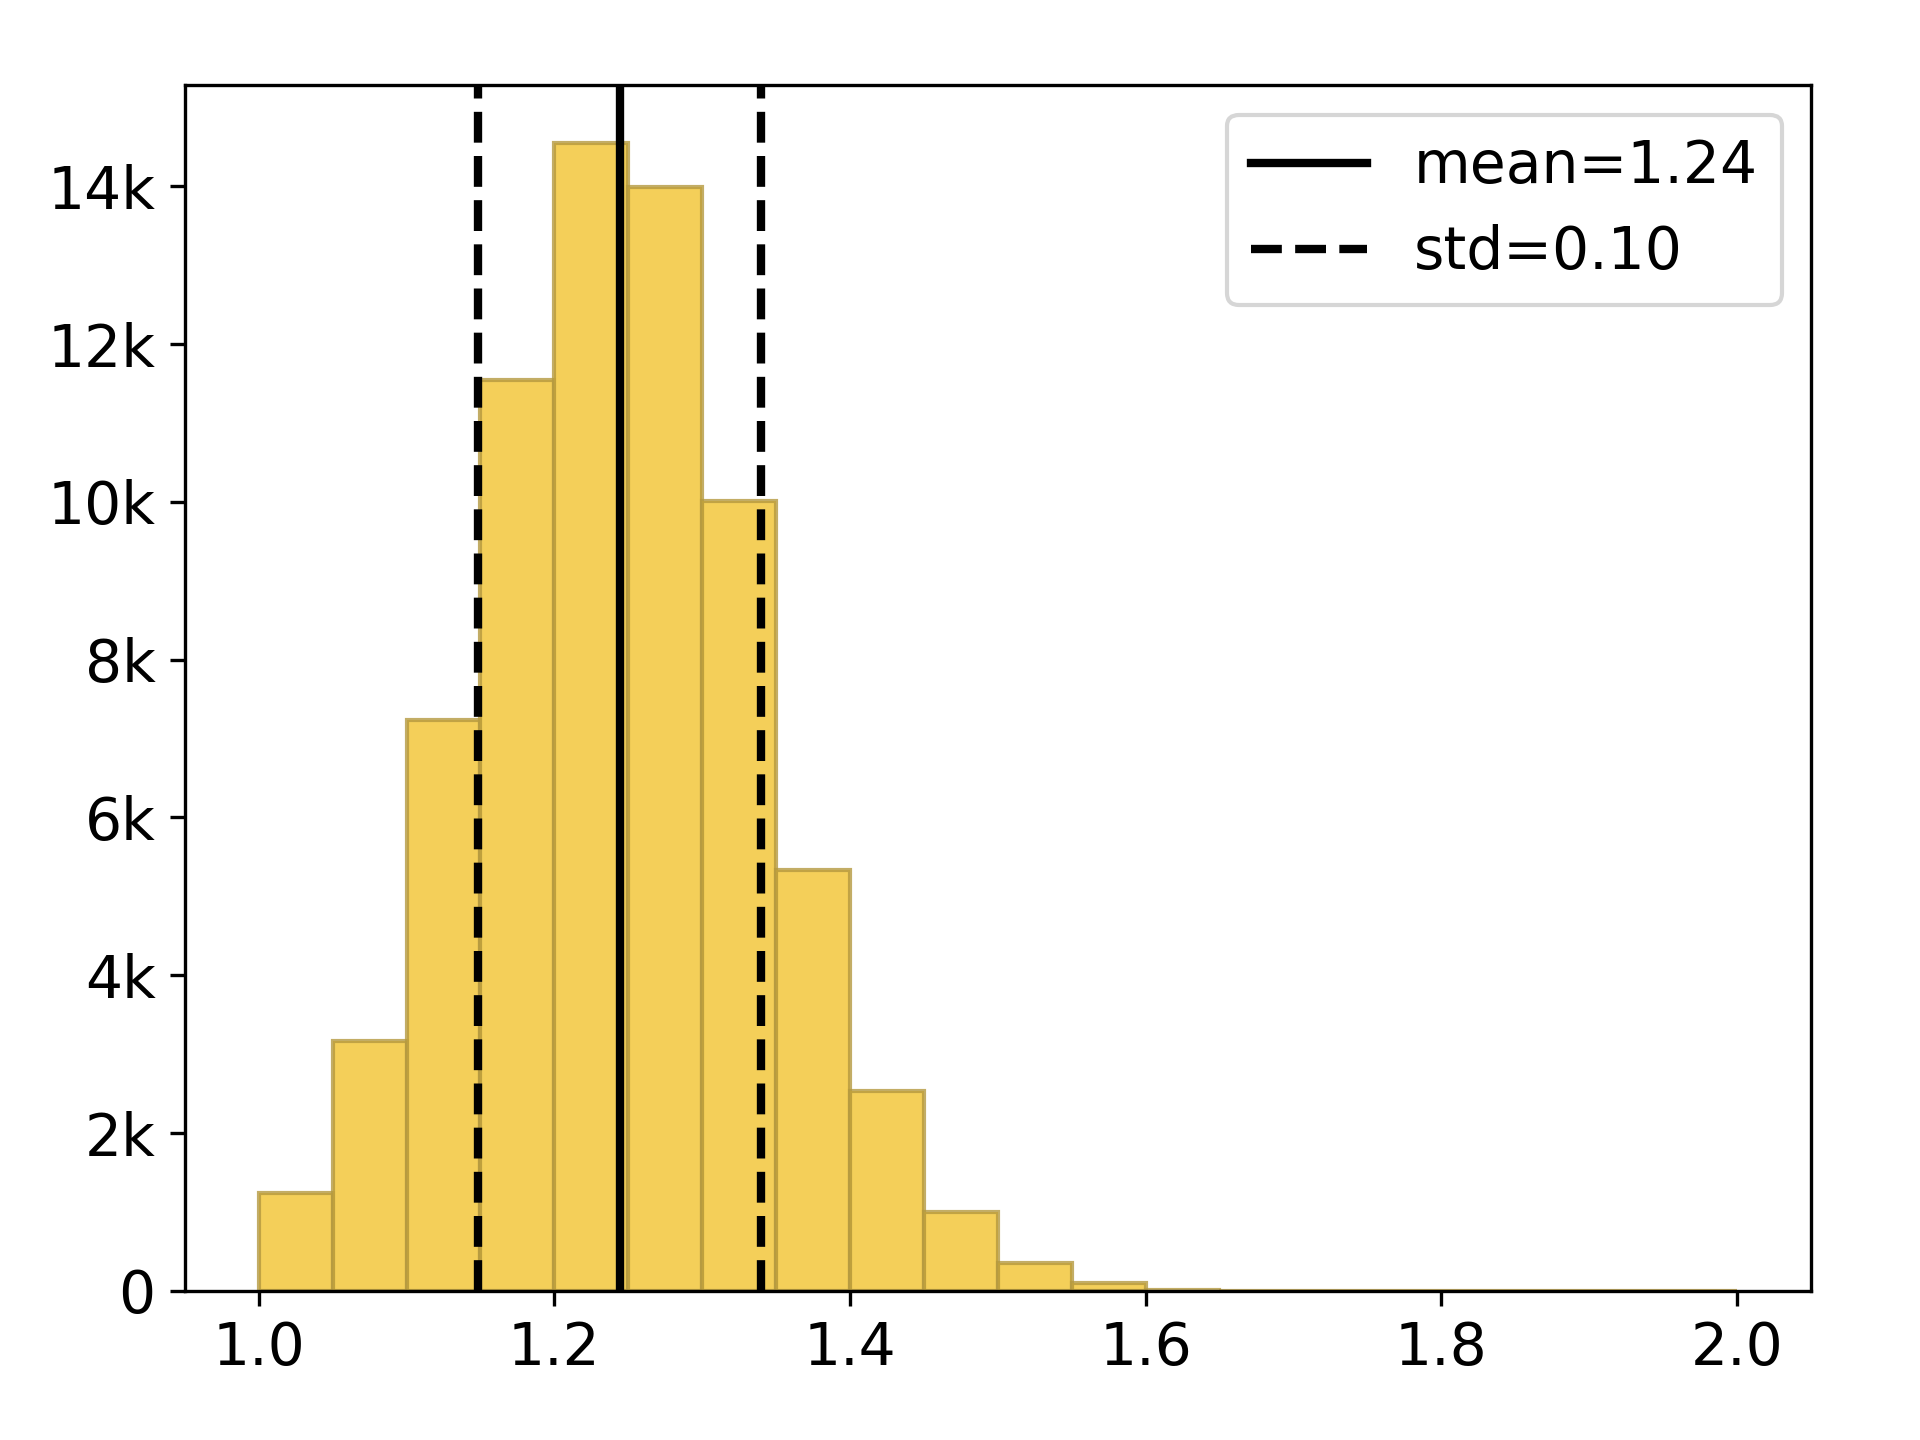
\includegraphics[width=\textwidth, trim=.25cm 0.25cm .25cm 0.25cm]{Resources/Images/Histogram/hist_1_b.png}
	\end{minipage}
	\begin{minipage}{.325\textwidth}
		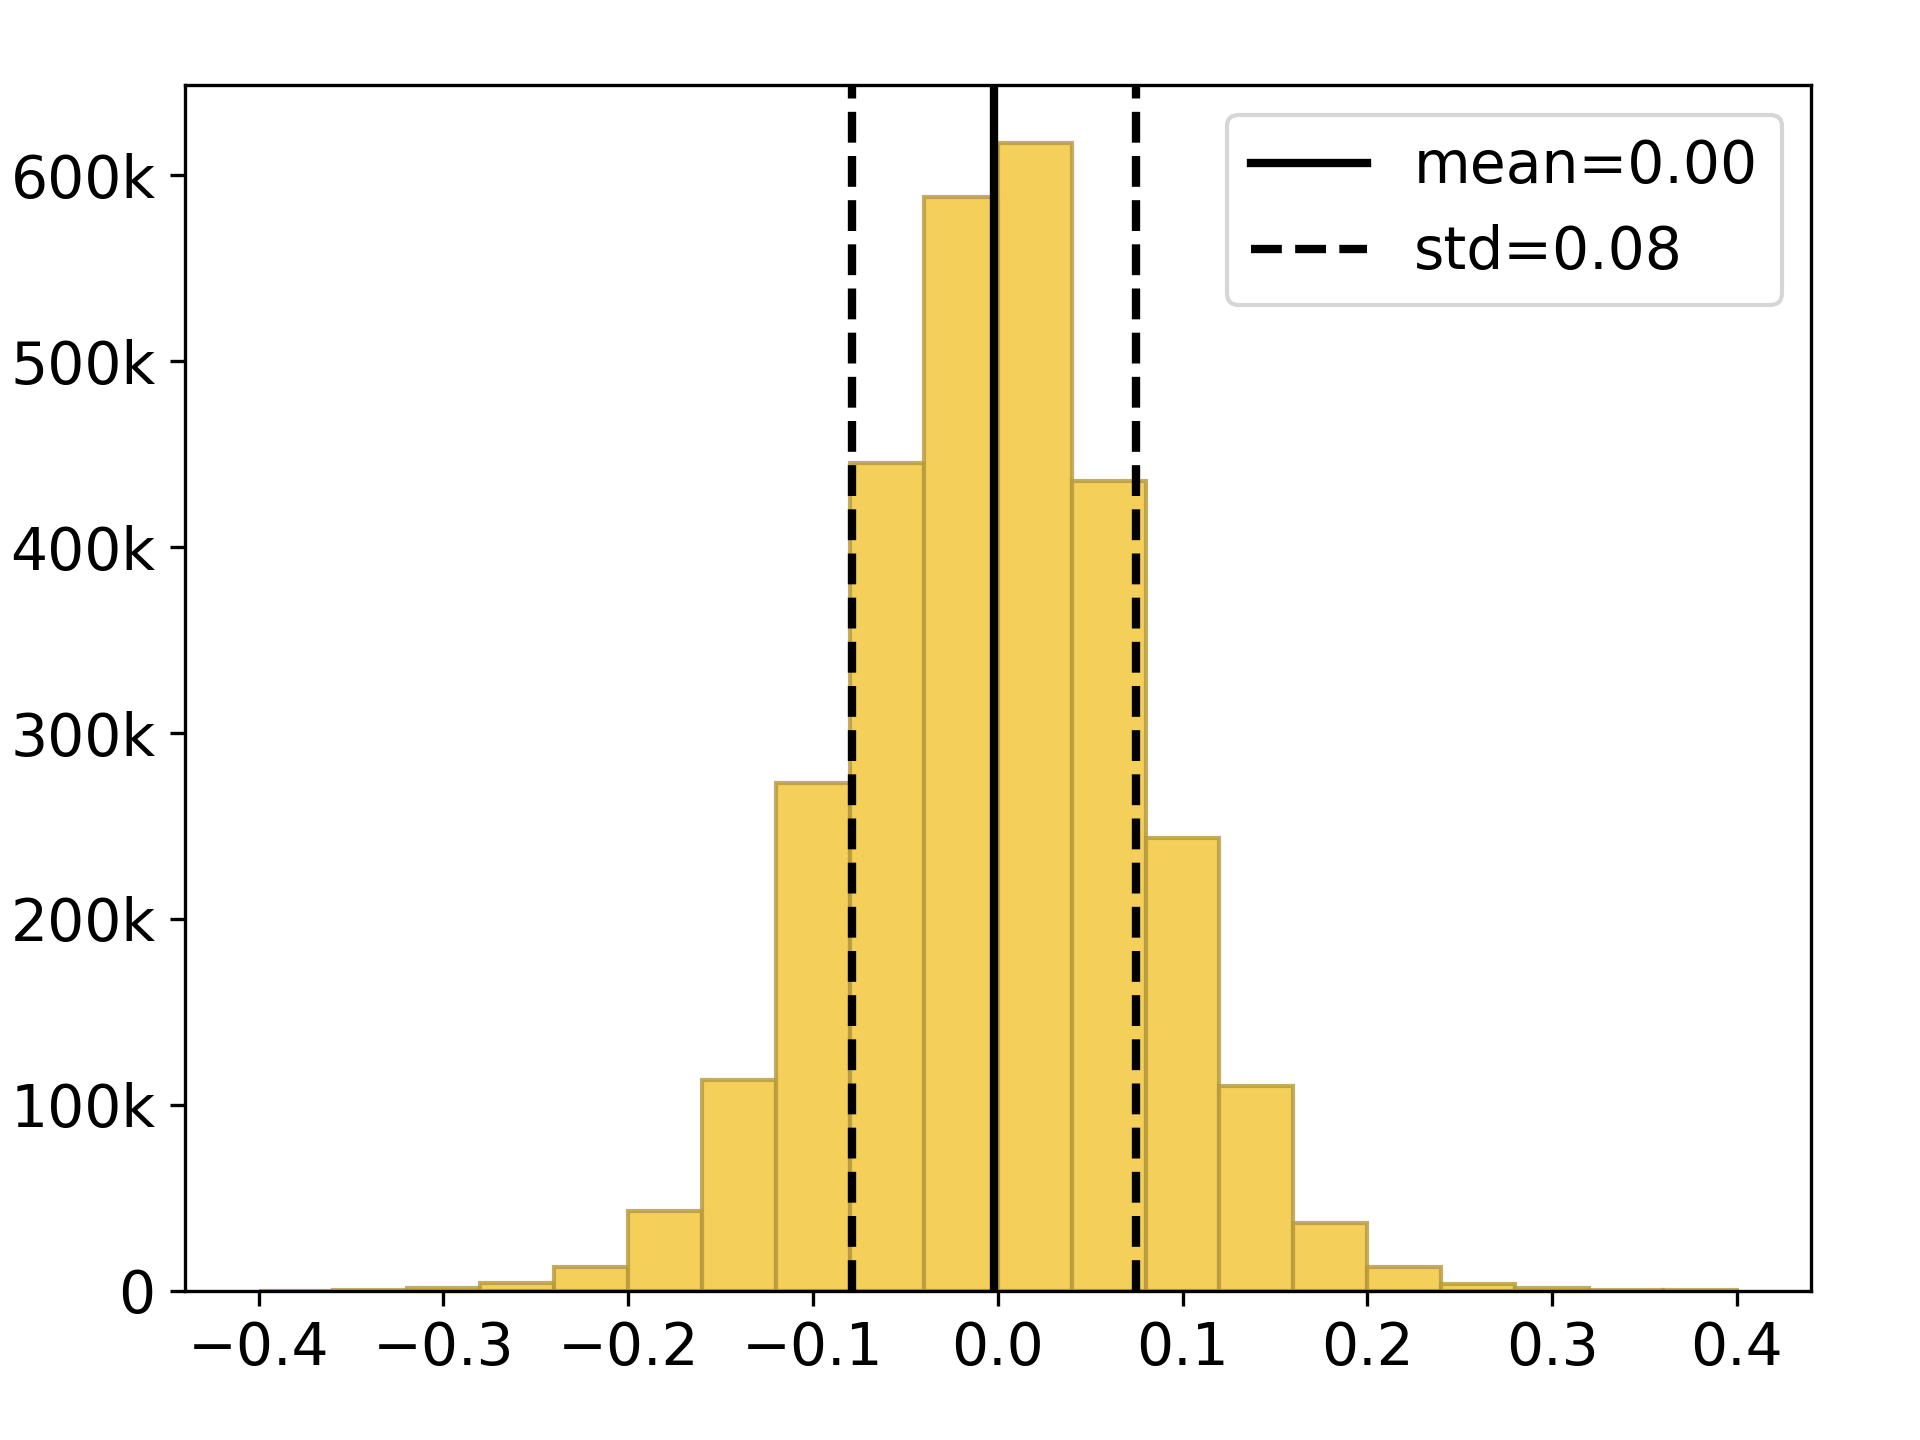
\includegraphics[width=\textwidth, clip, trim=.25cm 0.25cm .25cm 0.25cm]{Resources/Images/Histogram/hist_2_b.png}
	\end{minipage}
	\begin{minipage}{.325\textwidth}
		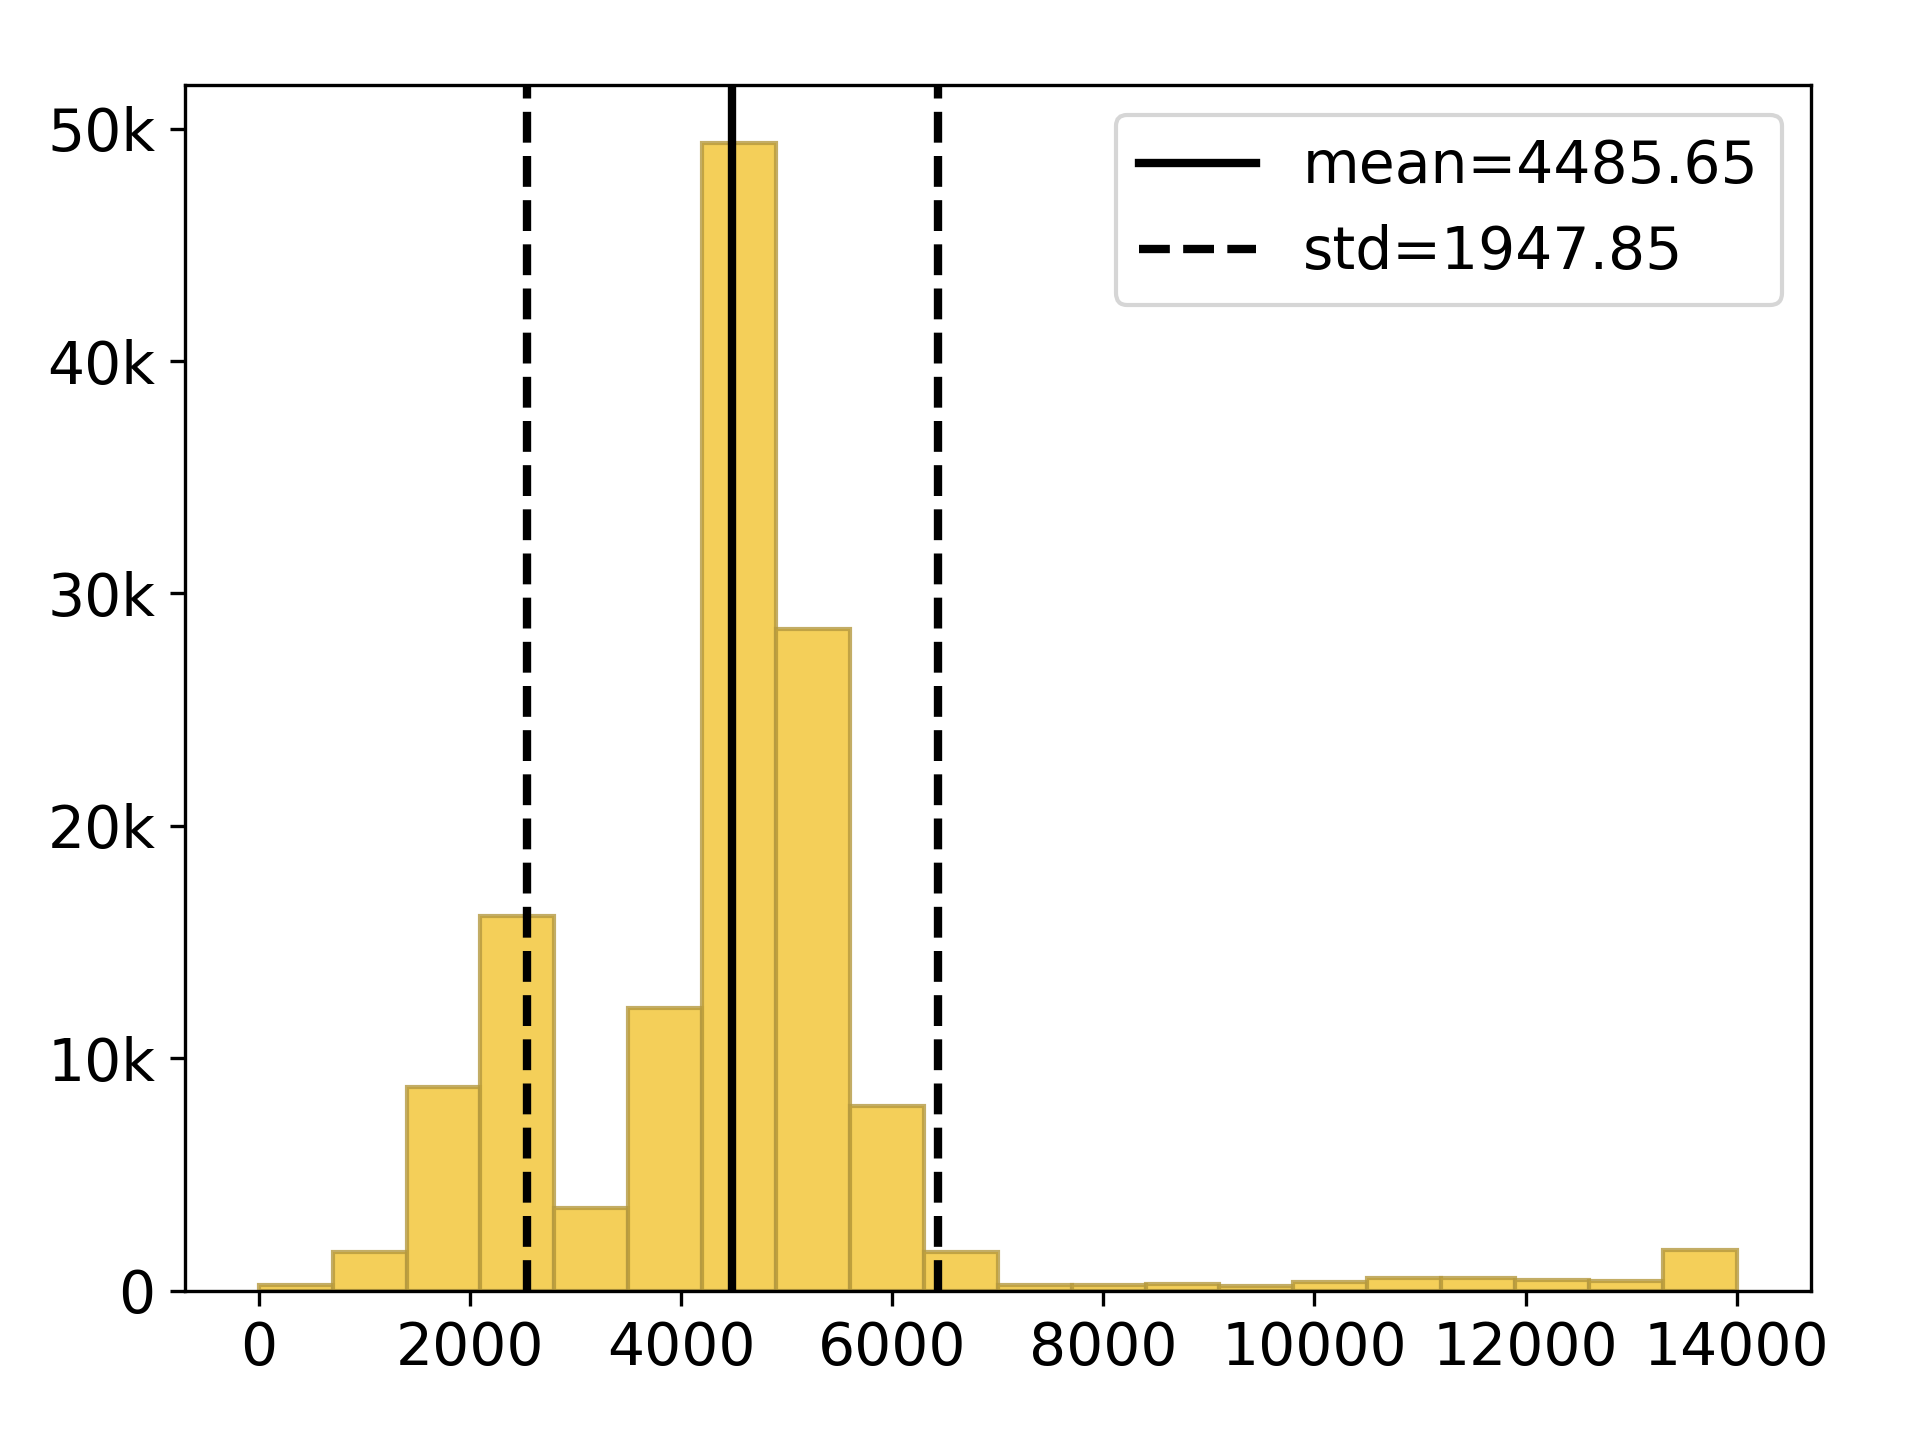
\includegraphics[width=\textwidth, trim=.25cm 0.25cm .25cm 0.25cm]{Resources/Images/Histogram/hist_3_b.png}
	\end{minipage}
	\caption{f.l.t.r. Histogram 1, Histogram 2, Histogram 3: Comparison of something (top row) and something different (bottom row)}
	\label{fig:images:histograms}
\end{figure}
